\documentclass[paper=letter, fontsize=12pt]{article}
\usepackage{geometry}
\geometry{margin=1in}
\usepackage{graphicx}
\graphicspath{{images/}}
\usepackage{amssymb}
\usepackage{enumitem}
\usepackage{amsmath}
\usepackage{mathrsfs}

%opening
\title{Compsci 571 HW6}
\author{Yilin Gao (yg95)}

\begin{document}

\maketitle
\section{Neural Networks and Universal Approximation Theorem}

\subsection{}

\begin{enumerate}[label=(\alph*)]
	\item The NN architecture is like following:
			
	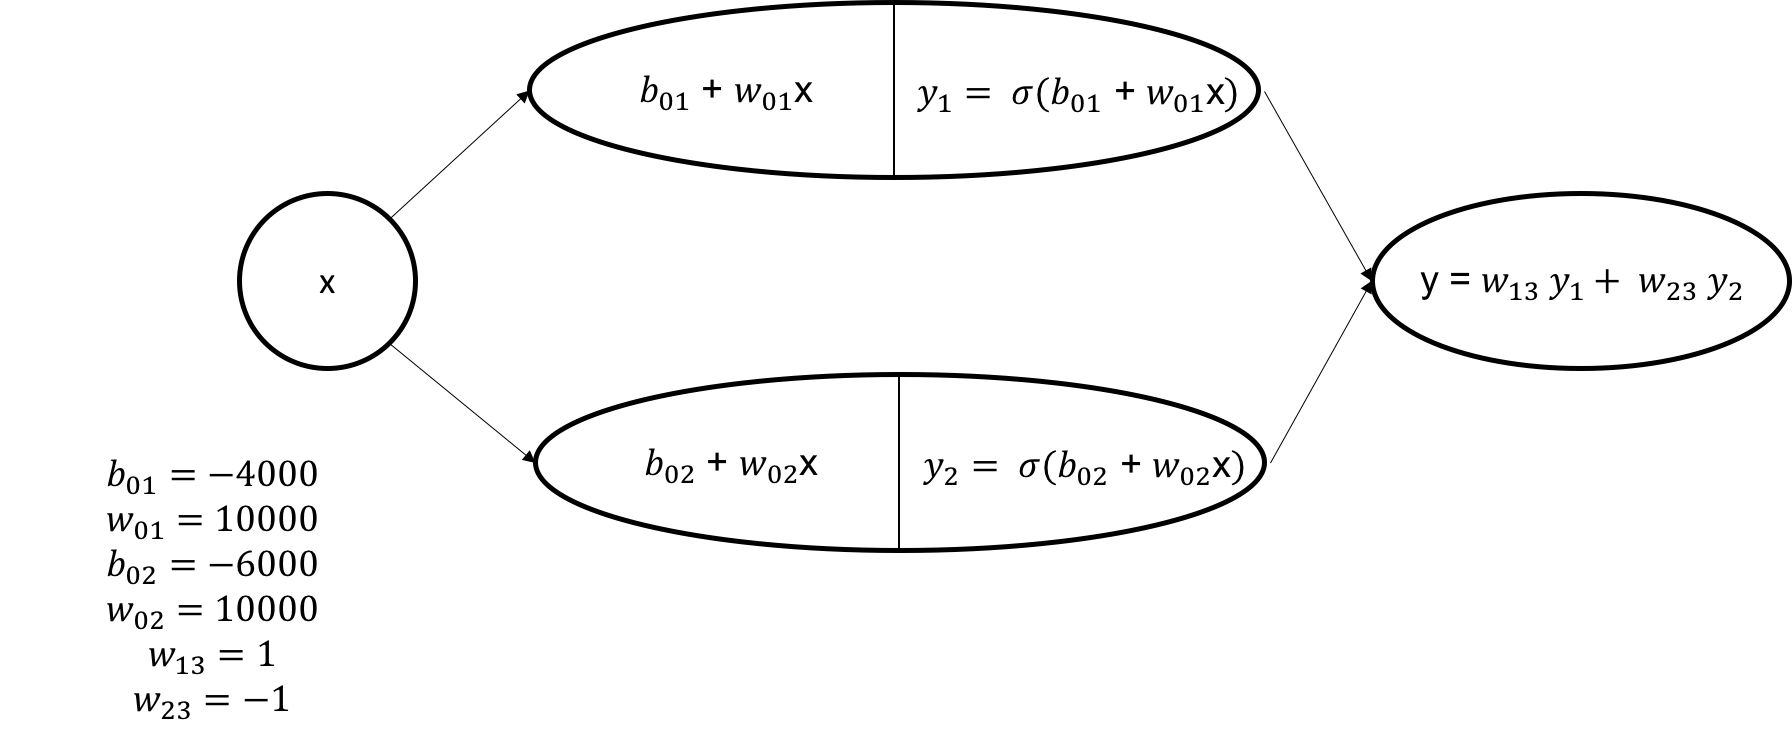
\includegraphics[scale=0.4]{q1a.png}
			 
	The implementation is in \verb|q1.ipynb|. The approximated function is as following:
	
	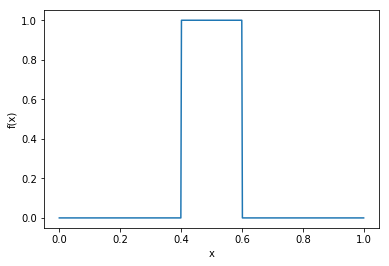
\includegraphics[scale=0.6]{q1a2.png}
			 
	The minimal number of hidden neurons is 2, because the bump is a combination of 2 step functions, and each neuron (with the sigmoid activation function) is able to approximate one step function with any given step direction, location and height.
	
	\item In the NN, $w_{01}$ determines the steepness of the step-up part of the bump, $w_{02}$ determines the steepness of the step-down part of the bump. $-\frac{b_{01}}{w_{01}}$ determines the step-up location, $-\frac{b_{02}}{w_{02}}$ determines the step-down location. And $w_{13}$ and $w_{23}$ determine the height of the bump.
\end{enumerate}

\subsection{}

\begin{enumerate}[label=(\alph*)]
	\item 
	
	\item 
	
	\item 
\end{enumerate}

\section{EM}

\section{Clustering}
\begin{enumerate}[label=(\alph*)]
	\item See the implementation in \verb|q3.ipynb|.
	
	\item See the implementation in \verb|q3.ipynb|.
	
	\item 
	
	\item
\end{enumerate}
\end{document}
